\section{Aufbau und Durchführung}
\label{sec:Durchführung}
\begin{figure}
    \centering
    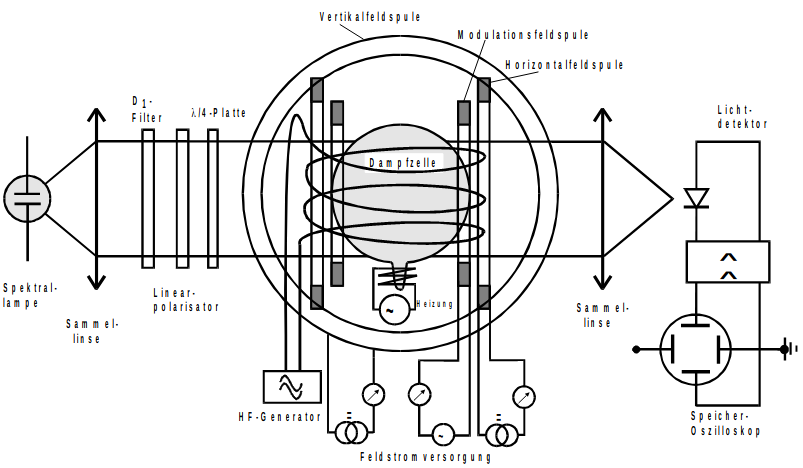
\includegraphics[width = 0.9 \textwidth]{pics/Aufbau.png}
    \caption{Versuchsaufbaut.
    Entmommen aus \cite{sample}}
    \label{fig:Ficken}
\end{figure}
Als Emissionsquelle dient eine Rb-Spektrallampe, die die gebrauchte Wellenlänge für die Übergänge liefert.
Die Sammellinse lässt das Licht parallel verlaufen, um die Verluste zu minimieren.
Fortan filtert der $D_1$-Filter die nicht gebrauchten Wellenlängen raus.
Der lineare Polarisator polarisiert das Licht linear, wonach die $\sfrac{\lambda}{4}$-Platte 
für eine reine rechts-zirkuläre Polarisation des Lichts, damit die richigen Auswahlregeln für die Übergänge gelten.
Danach tritt das Licht in drei Magnetfelder von drei Spulen ein. 
Einerseits sorgt ein vertikales Feld für die Kompensation der vertikalen Komponente des Erdmagnetfelds.
Die beiden horizontalen Spulen, wovon eine Sweep-Spule ist, sind zur Variation der Feldstärke bei verschiedenen 
Frequenzen des HF-Generators, womit die Resonanzen für die induzierte Emission getroffen werden.
Die zweite Sammellinse bündelt das Licht, damit eine möglichst hohe Intensität an dem Lichtdetektor ankommt.
Das Signal wird im $x\text{-}y$-Modus am Oszilloskop dargestellt.\\
Zunächst wird die zur Minimierung der Umwelteinflüsse abgedeckte Aufbaut gedreht, so dass die horizontale Feldkomponente der Erde (anti-)parallel zu den horizontalen Felder 
der Apperatur steht. 
Danach wird die vertikale Komponente des Erdfeldes mittels vertikalen Spule kompensiert, damit
der Peak auf möglichst schmal ist.
Nachdem das Erdmagnetfeld berücksichtigt wurde, wird der HF-Generator angeschaltet, womit die $D_1$-Übergänge der beiden Isotope
am Oszilloskop ersichtlich werden.
Die  Frequenzen wurden im Bereich von 100 bis $\qty{1000}{\kilo\hertz}$ in 10 Schritten varriert.
Mittels der Sweep-Spule und der festen horizontalen Spule werden die Peaks gesucht und der Strom, welcher die Magnetfelder beider Spulen induziert, notiert.
